% !TeX program = xelatex
\documentclass{beamer}
\usepackage{etex} % fixes new-dimension error
%-------------- template --------------------------------------------------
\usetheme{metropolis}
\metroset{block=fill}
%\usetheme{Boadilla}

% Configuring the foot line
\setbeamertemplate{footline}
{
  \leavevmode%
  \hbox{%
  \begin{beamercolorbox}[wd=.4\paperwidth,ht=2.25ex,dp=1ex,center]{author in head/foot}%
    \usebeamerfont{author in head/foot}\insertshortauthor
  \end{beamercolorbox}%
  \begin{beamercolorbox}[wd=.5\paperwidth,ht=2.25ex,dp=1ex,center]{title in head/foot}%
    \usebeamerfont{title in head/foot}\insertsection
  \end{beamercolorbox}%
  \begin{beamercolorbox}[wd=.1\paperwidth,ht=2.25ex,dp=1ex,right]{date in head/foot}%
    \insertframenumber{} / \inserttotalframenumber\hspace*{2ex} 
  \end{beamercolorbox}}%
  \vskip0pt%
}
% No configuration symbols
\makeatother
\setbeamertemplate{navigation symbols}{}
%----------------------------------------------------------------------------
\usepackage{graphicx,amsmath}
\usepackage{stmaryrd} % cf. interleave
\usepackage{booktabs}
\usepackage{amscd}
\usepackage{multicol}
\usepackage[absolute,overlay]{textpos}
\usepackage{alltt}
\usepackage{proof}
\usepackage{subcaption}
\usepackage{tikz}
\usepackage{tikz-cd}
\usepackage[new]{old-arrows}
\usepackage[all]{xy}
\usepackage{pgfplots}
\usepackage{textcomp}
\usepackage{listings}
\usetikzlibrary{arrows.meta, calc, fit, tikzmark}


\AtBeginSection[]
{
    \begin{frame}
        \frametitle{Table of Contents}
        \tableofcontents[currentsection]
    \end{frame}
}
\author[Renato Neves]{Renato Neves}

% logos of institutions
\titlegraphic{
  \begin{textblock*}{5cm}(7.8cm,7.45cm)
     \includegraphics[scale=0.044]{images/uminho.png}\hspace*{.85cm}~%
  \end{textblock*}
  \begin{textblock*}{5cm}(9.8cm,7.45cm)
    \includegraphics[scale=0.4]{images/haslab.pdf}
  \end{textblock*}
}

\input{macros}
% No date
\date{}

\begin{document}

\title{Cyber-Physical Computation}

\frame[plain]{\titlepage}

\section{Cyber-Physical systems}

\begin{frame}{\underline{Cyber-Physical} systems}

\begin{center}
  \small{\alert{Digital} devices that interact with their \alert{physical} environment}
\end{center}
  
\begin{textblock*}{5cm}(1.2cm,1.5cm)
\includegraphics[scale=0.205]{images/aviao.jpg} 
\end{textblock*}


\begin{textblock*}{5cm}(1.2cm,5.6cm)
\includegraphics[scale=0.2]{images/pace.jpg} 
\end{textblock*}


\begin{textblock*}{5cm}(6.6cm,5.6cm)
\includegraphics[scale=0.32]{images/nuclear.jpg}
\end{textblock*}

\begin{textblock*}{5cm}(6.6cm,1.5cm)
\includegraphics[scale=0.0357]{images/beetle.jpg} 
\end{textblock*}
\end{frame}

\begin{frame}{Another example of a cyber-physical system}
  \centering
  \href{https://www.youtube.com/watch?v=_qwLHlVjRyw&t=82s}{
    \includegraphics[scale=0.3]{images/shuttle.png}
  }
\end{frame}

\begin{frame}{The three ingredients of cyber-physical systems}

        Concurrency

        Communication

        \alert{Hybrid interaction}
\end{frame}

\lstset{
showstringspaces=false,
keywordstyle=\color{blue},
basicstyle=\fontsize{08.5}{10}\ttfamily,
emph={while,do,if,diff,for,exit,blue,unif,then,else,wait,bernoulli,exp,normal,sqrt,cos},emphstyle=\color{blue},
breaklines=true,
escapeinside={*@}{*@}
}


\begin{frame}[fragile]{Computer Science meets Analysis}
 \centering
 \scalebox{0.7}{
         \hspace{-0.8cm}
 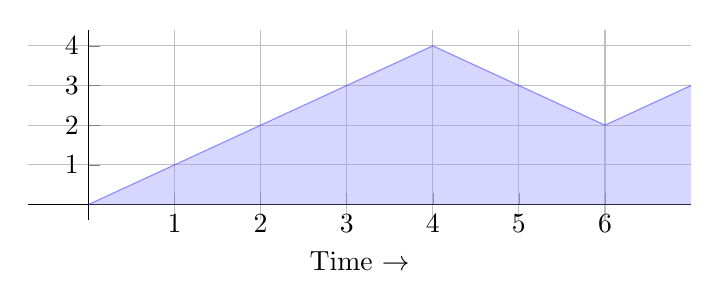
\begin{tikzpicture}
   \begin{axis}[ width=10cm, height=4cm, x axis line style={}, grid =
     major ,y axis line style={},
     title={}, xtick =
     {0,1,2,3,4,5,6} , xmax=7, axis lines*=center,
     ytick={0,1,2,3,4,5,6}, xlabel={Time $\rightarrow$}, ylabel={},
     xlabel near ticks, ylabel near ticks] \addplot [color=blue,
     domain = 0:5, fill = blue!40!white, opacity=0.4 ] coordinates {
     (0,0) (2,2) (4,4) (6,2) (8,4) (8,0)};
 \end{axis}
 \end{tikzpicture}}

 \begin{center}
 \begin{minipage}{0.8\textwidth}
 \begin{lstlisting}
  while true do {
        if v <= 2 
           then v' = 1 for 2 
           else v' = -1 for 2
        }
 \end{lstlisting}
 \end{minipage}
\end{center}
\end{frame}

\begin{frame}[fragile]{A particle and its orbital trajectory -- what can go wrong?}
        \begin{lstlisting}
        x := -1; v := 0; a := 1;
        while true do {
             if x <= 0 
                then a := 1 
                else a :=-1
             x' = v, v' = a for 0.5
        }
        \end{lstlisting}
\end{frame}

\begin{frame}{Cyber-Physical \underline{Computation}}

\centering
\includegraphics[scale=0.15]{images/hitchhiker.jpg} 

What is actually \alert{computable} ?
\end{frame}

\begin{frame}{Cyber-Physical \underline{Computation}}

  \begin{minipage}[0.3\textheight]{\textwidth}
  \begin{columns}[c]
  \begin{column}{0.6\textwidth}
    \emph{Genesis}: David Hilbert and its \emph{\alert{Entscheidungsproblem} (\emph{circa} 1928)}
  \end{column}
  \begin{column}{0.2\textwidth}
    \includegraphics[scale=0.15]{images/Hilbert.jpg}
  \end{column}
  \end{columns}
  \end{minipage}

  \vspace{0.5cm}
  Led to the first models of computation (\emph{circa} 1936)
  \begin{itemize}
  \item Turing machines: state-based, part of \alert{automata} theory
  \item $\lambda$-calculus: functional, prototypical
          \alert{programming} language
  \end{itemize}
\end{frame}

\begin{frame}{Church-Turing \underline{Thesis}}
        \begin{minipage}[0.3\textheight]{\textwidth}
        \begin{columns}[c]
        \begin{column}{0.6\textwidth}
                \alert{Computable} if encodable as a Turing
                machine or (equivalently) as a $\lambda$-term
        \end{column}
        \begin{column}{0.2\textwidth}
          \includegraphics[scale=0.35]{images/ChurchTuring.jpg}
        \end{column}
        \end{columns}
        \end{minipage}
\end{frame}
\section{Course contents}


\begin{frame}{Contents of the course pt. I}
  We will study diverse models of cyber-physical computation
  \begin{itemize}
  \item (timed) automata,
  \item a hybrid while-language,
  \item $\lambda$-calculus with computational effects (\alert{monads!})
  \end{itemize}

  \pause
  and often make detours through the \alert{mathematical foundations} of automata and
  programming language theory \dots
\end{frame}

\begin{frame}{Contents of the module pt. II}
  We will get accquainted with diverse tools
  \begin{itemize}
          \item \textbf{Uppaal} verification of real-timed systems modelled by (networks of) timed automata
          \item \textbf{Lince} agile analysis of cyber-physical systems modelled by a hybrid
          while-language
  \item \textbf{Haskell} a platform to study $\lambda$-calculus with effects
  \end{itemize}
\end{frame}

\begin{frame}{How deep will we go into the rabbit hole?}

  \begin{minipage}[1\textheight]{\textwidth}
  \begin{columns}[c]
  \begin{column}{0.8\textwidth}

    Our learning path will intersect theory and practice \dots
  
    from basics to the state-of-the-art \dots

    we will face the turmoils of current limitations \dots

    and see what challenges lie ahead 
  \end{column}
  \begin{column}{0.2\textwidth}
    
    \includegraphics[scale=1.4]{images/rabbit.png}
  \end{column}
  \end{columns}
  \end{minipage}

\end{frame}

\section{Logistics}

\begin{frame}{Assessment}
  Two assignments (about the modelling and analysis of cyber-physical systems)
\end{frame}

\begin{frame}{Materials and contacts}
  Relevant class material and announcements posted on the website

  \url{https://haslab.github.io/MFP/}

  e-mail: \href{mailto:nevrenato@di.uminho.pt}{nevrenato@di.uminho.pt}

  office hours: tuesday afternoon (please send an email the day before if you wish to meet)
\end{frame}

\nocite{rajkumar10,lee06}
\bibliographystyle{amsalpha}
\bibliography{biblio.bib}
\end{document}
